\chapter{Creating a Repository (Stratum~0)}
\label{sct:createrepo}

\cvmfs\ is a file system with a single source of (new) data.
This single source, the repository \emph{Stratum 0}, is maintained by a dedicated \emph{release manager machine}.
A read-writable copy of the repository is available on the release manager machine.
The \cvmfs\ server tool kit is used to \emph{publish} the current state of the repository on the release manager machine.
Publishing is an atomic operation.

All data stored in \cvmfs\ have to be converted into a \cvmfs\ \emph{repository} during the process of publishing.
The \cvmfs\ repository is a form of content-addressable storage.
Conversion includes creating the file catalog(s), compressing new and updated files and calculating content hashes.
Storing the data in a content-addressable format results in automatic file de-duplication.
It furthermore simplifies data verification and it allows for file system snapshots.

In order to provide a writable \cvmfs\ repository, \cvmfs\ uses a union file system that combines a read-only \cvmfs\ mount point with a writable scratch area~\cite{unionfs04,aufs}.
Figure~\ref{fig:installwebserver} outlines the process of publishing a repository.

\begin{figure}[h]
	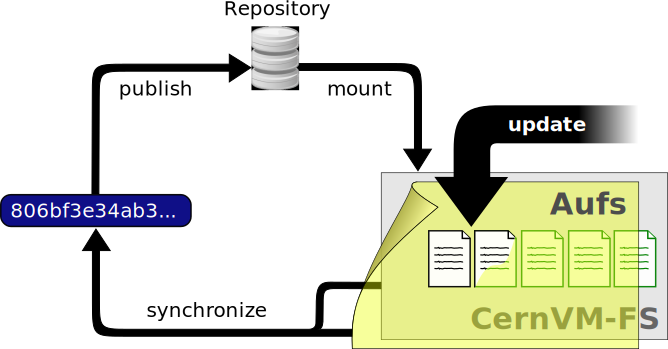
\includegraphics[width=\textwidth]{figures/update_process.png}
	\caption{Updating a mounted \cvmfs\ repository by overlaying it with a copy-on-write \aufs\ volume. 
		Any changes will be accumulated in a writable volume (yellow) and can be synchronized into the \cvmfs\ repository afterwards. 
		The file catalog contains the directory structure as well as file metadata, symbolic links, and secure hash keys of regular files. 
		Regular files are compressed and renamed to their cryptographic content hash before copied into the data store.}
	\label{fig:installwebserver}
\end{figure}

\section{Publishing a new Repository Revision}
\label{sct:repoupdate}

Since the repositories may contain many file system objects\footnote{For ATLAS, for example, ``many'' means order of $10^7$ file system objects (\ie number of regular files, symbolic links, and directories).}, we cannot afford to generate an entire repository from scratch for every update.
Instead, we add a writable file system layer on top of a mounted read-only \cvmfs\ repository using the union file system \aufs~\cite{aufs}.
This renders a read-only \cvmfs\ mount point writable to the user, while all performed changes are stored in a special writable scratch area managed by \aufs.
%One could see the result as a virtual version of the \emph{shadow tree} we used for updating repositories in previous versions of \cvmfs.
A similar approach is used by Linux Live Distributions that are shipped on read-only media, but allow \emph{virtual} editing of files where changes are stored on a RAM disk.

If a file in the \cvmfs\ repository gets changed, \aufs\ first copies it to the writable volume and applies any changes to this copy (copy-on-write semantics).
\aufs\ will put newly created files or directories in the writable volume as well.
Additionally it creates special hidden files (called \emph{white-outs}) to keep track of file deletions in the \cvmfs\ repository.

Eventually, all changes applied to the repository are stored in \aufs's scratch area and can be merged into the actual \cvmfs\ repository by a subsequent synchronization step.
Before the actual synchronization step takes place, no changes are applied to the \cvmfs\ repository.
Therefore, any unsuccessful updates to a repository can be rolled back by simply clearing the writable file system layer of \aufs.

\section{Requirements for a new Repository}
\label{sct:newreporequirements}

In order to create a repository, the server and client part of \cvmfs\ must be installed on the release manager machine.
Furthermore your machine should provide an \aufs\ enabled Kernel as well as a running \texttt{Apache2} web server.
Currently we support Scientific Linux 5 and 6 as well as Ubuntu 12.04 distributions.
Please note, that Scientific Linux 6 \emph{does not} ship with an \aufs\ enabled kernel, therefore we provide a compatible patched kernel as RPMs (see Appendix~\ref{apx:rpms}).

%Special care should be taken for the mount point of \cvmfs\ repositories.
%From the point of view of the file system, repositories are relocatable.
%However, many software installation tools hard-code the full path and therefore break relocatability on the application level.
%In effect, repositories have to be mounted at the same location that was used to install it on the release manager machine.
%By convention, \cvmfs\ repositories are mounted using their fully qualified repository name under \texttt{/cvmfs}, for instance at \texttt{/cvmfs/atlas.cern.ch}.

\section{\cvmfs\ Repository Creation and Updating}
\label{sct:repocreateandupdate}
The \cvmfs\ server tool kit provide the versatile \texttt{cvmfs\_server} utility in order to perform all operations related to repository creation, updating, deletion, replication and inspection.
Please run it without any parameters to get a short documentation of its commands.

\subsection{Repository Creation}
\label{sct:repocreation}

A new repository is created by \texttt{cvmfs\_server mkfs}:
\begin{verbatim}
  cvmfs_server mkfs my.repo.name
\end{verbatim}
The utility will then ask you for a user that should act as the owner of the repository and afterwards create all the infrastructure for the new \cvmfs\ repository.
Additionally it will create a reasonable default configuration and generate a new release manager certificate and software signing key. 
You'll have to distribute the public key in /etc/cvmfs/keys/my.repo.name.pub to all your client machines.
The \texttt{cvmfs\_server} utility will use \texttt{/srv/cvmfs} as storage location.
In case you want to use a separate hard disk, you should mount it there upfront.

Once created, you should see your repository mounted under \texttt{/cvmfs/my.repo.name} containing only a single file called \texttt{new\_repository}.
Following this step, you can produce the first revision by going through the repository update procedure described in the next section.

\subsection{Repository Update}
Typically a repository publisher does the following steps in order to create a new revision of a repository:
\begin{enumerate}
	\item Run \texttt{cvmfs\_server transaction} to switch to a copy-on-write enabled \cvmfs\ volume
	\item Make the necessary changes to the repository, \eg add new directories, patch certain binaries, \dots
	\item Test the software installation
	\item Do one of the following:
	\begin{itemize}
		\item Run \texttt{cvmfs\_server publish} to finalize your new repository revision \emph{or}
		\item Run \texttt{cvmfs\_server abort} to clear all changes and start over again
	\end{itemize}
	\item Make the web server serve the new version of the repository directory.
\end{enumerate}

\cvmfs\ supports to have more than one repository on a single server machine.
In case of a multi-repository host, you need to specify which repository you want to operate on, when running the \texttt{cvmfs\_server} utility commands.
Additionally you should run \texttt{cvmfs\_server resign} every 30 days to update the signatures of the repository.
